\section{\texttt{docker-compose}を使用したアプリケーションのデプロイ(Overleafを例として)}

\texttt{docker-compose}は,Docker公式が提供するツールであり,複数のコンテナを用いたDockerアプリケーションを定義・管理するために使用される.YAMLファイルを使用して,アプリケーションに必要なすべてのサービスを設定し,単一のコマンドでサービスの起動や停止ができる.この機能は,Webサービス,データベース,キャッシュなど,複数の相互依存するサービスを持つアプリケーションに特に有用である.

Overleafは,リアルタイムの共同編集とコンパイル機能を提供するオンライン \LaTeX エディタである.そのCE版はオープンソースとして公開されており,自己ホスティングが可能である.公式のサイトでは多人数でのコラボレーション機能を利用するには課金が必要だが,CE版をローカルサーバーにデプロイすれば,この制約なしに利用できる.

\subsection{\texttt{docker-compose}を用いたOverleafのデプロイ}
\texttt{docker-compose}は関連する設定情報をディレクトリ単位で管理する.本チュートリアルで使用する設定ファイルは以下のリポジトリから取得する:

\begin{lstlisting}[language=bash]
git clone https://github.com/watashihame/25OnCampusJob.git
\end{lstlisting}

\paragraph{リポジトリを使用しない方法}
\begin{enumerate}
\item 作業ディレクトリの作成
\begin{lstlisting}[language=bash]
mkdir overleaf-test
cd overleaf-test
\end{lstlisting}

\item Overleaf設定ファイルの取得
\begin{lstlisting}[language=bash]
wget https://raw.githubusercontent.com/watashihame/25OnCampusJob/refs/heads/main/overleaf-test/docker-compose.yml
\end{lstlisting}
\end{enumerate}

\paragraph{設定ファイルの解説}
Overleafの設定は\texttt{./overleaf-test}の\texttt{docker-compose.yml}ファイルによって記述されている.
このファイルは3つのコンテナ(\texttt{sharelatex},\texttt{mongo},\texttt{redis})を定義しており,起動順序は\texttt{depends\_on}(依存関係)によって制御されている.

主要なカスタマイズ項目:
\begin{itemize}
\item ポートマッピング:\texttt{sharelatex}サービスの\texttt{ports}設定(例:\texttt{"80:80"}→\texttt{"8808:80"})
\item 環境変数:各サービスごとの設定パラメータ
\item データ保存先(ボリューム):
  \begin{itemize}
  \item \texttt{./sharelatex\_data}: プロジェクトファイルとコンパイル結果(Project files and build artifacts)
  \item \texttt{./mongo\_data}: MongoDBデータベース(Database storage)
  \item \texttt{./redis\_data}: Redisキャッシュ(In-memory data store)
  \end{itemize}
\end{itemize}

\paragraph{注意}
\begin{itemize}
\item データ保存先の変更は\texttt{volumes}設定を編集する
\item 本設定ファイルは簡略化版であり,HTTPS対応やNginxリバースプロキシなどの高度な設定が必要な場合は,\href{https://github.com/overleaf/overleaf/tree/main}{公式リポジトリ}を参照すること
\item Overleafは現在docker-composeを使用したセルフホスティングを推奨していない(あくまでデモンストレーション目的での使用を想定)
\end{itemize}

設定が完了したら,以下のコマンドでOverleafを起動する:

\begin{lstlisting}[language=bash]
docker compose up -d
\end{lstlisting}

正常に起動すると,以下のようなメッセージが表示される:

\begin{lstlisting}[language=bash]
$ docker compose up -d
[+] Running 3/3
 |!\checkmark!| Container mongo-test       Healthy   10.7s
 |!\checkmark!| Container redis-test       Started    0.2s
 |!\checkmark!| Container sharelatex-test  Started   10.9s
\end{lstlisting}

停止する場合は以下のコマンドを使用する:

\begin{lstlisting}[language=bash]
docker compose down
\end{lstlisting}

また,再起動する場合は以下のコマンドを使用する:

\begin{lstlisting}[language=bash]
docker compose restart
\end{lstlisting}

\subsection{Overleafサービスの初期設定}

起動後,\texttt{http://localhost:8808} にアクセスすると,Overleafの管理画面に入ることができる.

\begin{figure}[H]
    \centering
    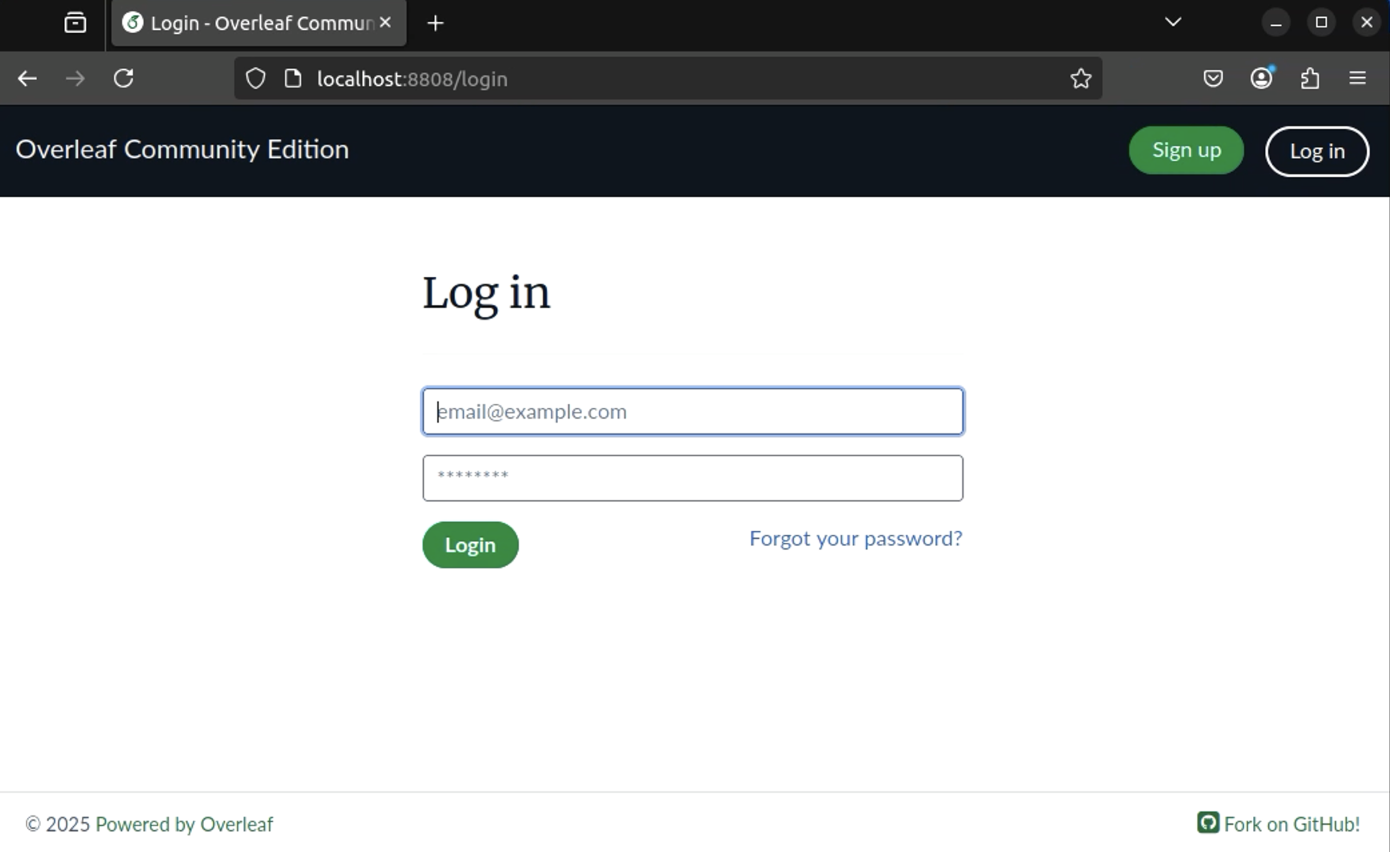
\includegraphics[width=0.8\linewidth]{images/Pasted image 20250307155416.png}
\end{figure}

管理者アカウントを作成するため,\\ \texttt{http://localhost:8808/launchpad} にアクセスする.

\begin{figure}[H]
    \centering
    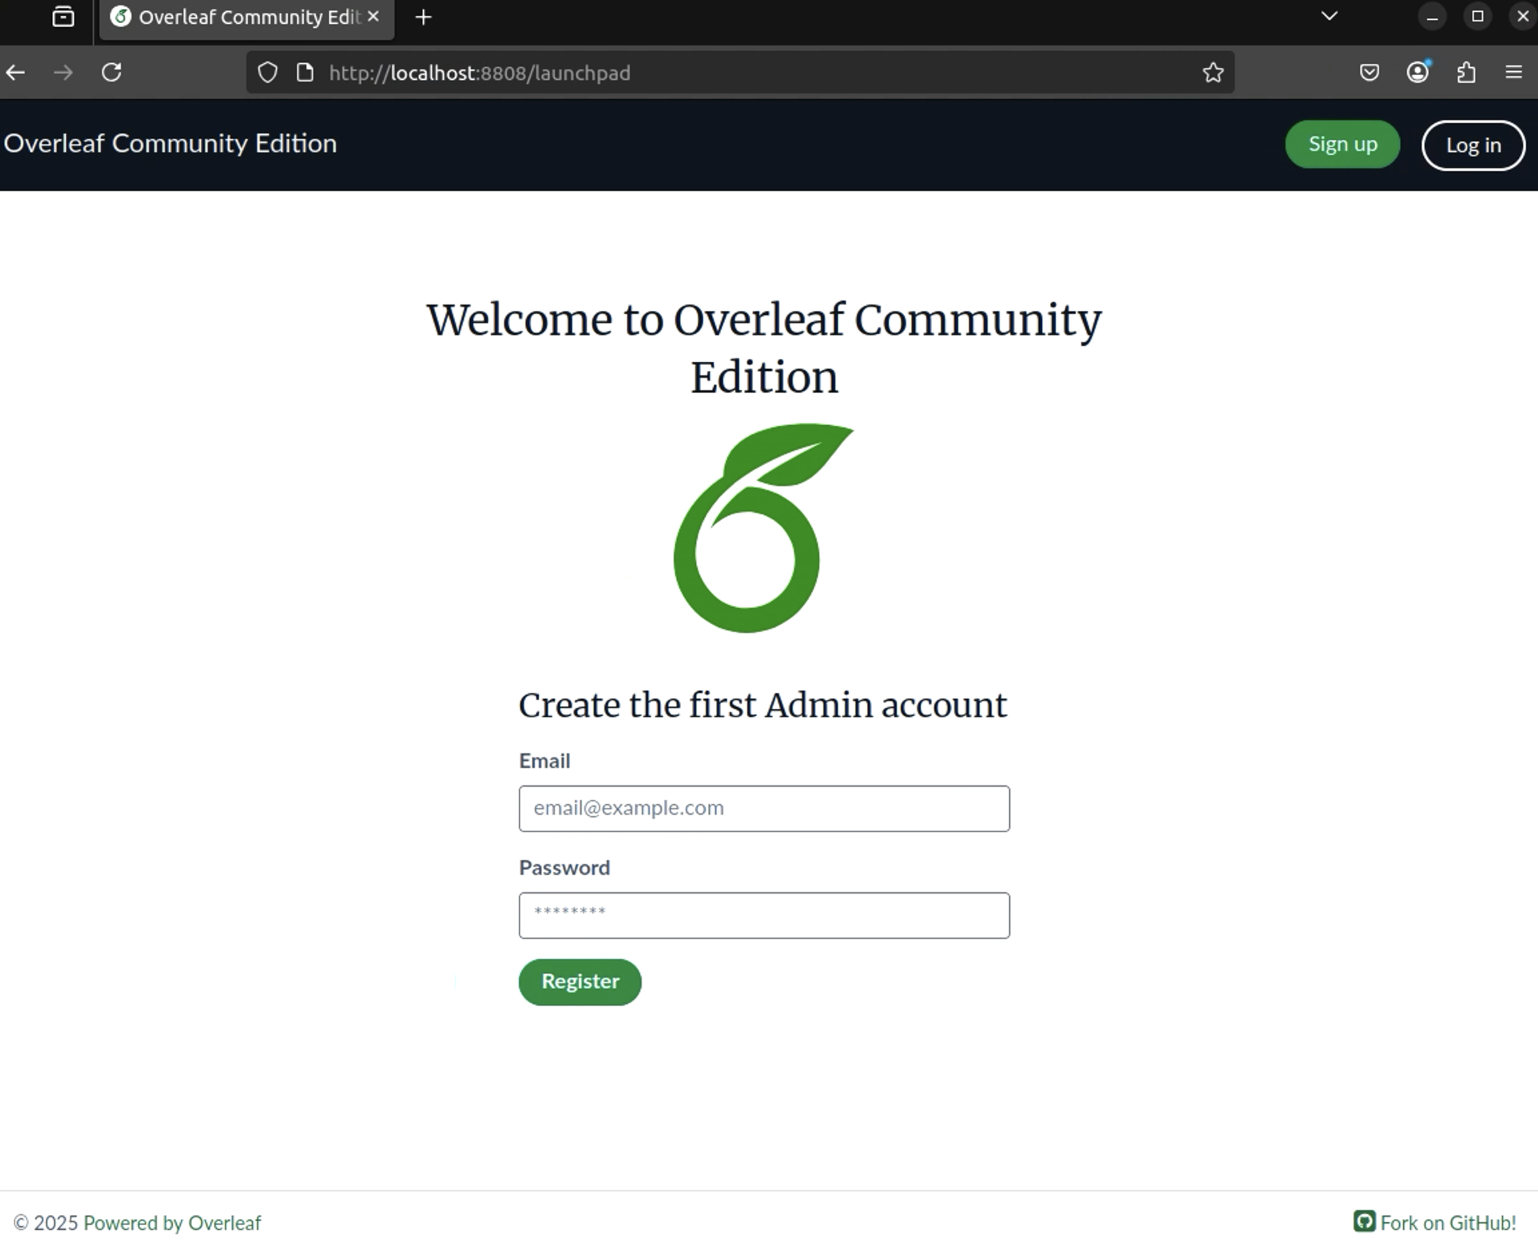
\includegraphics[width=0.8\linewidth]{images/Pasted image 20250307160444.png}
\end{figure}

登録後,ログイン画面に遷移し,作成したアカウントでログインできる.

\begin{figure}[H]
    \centering
    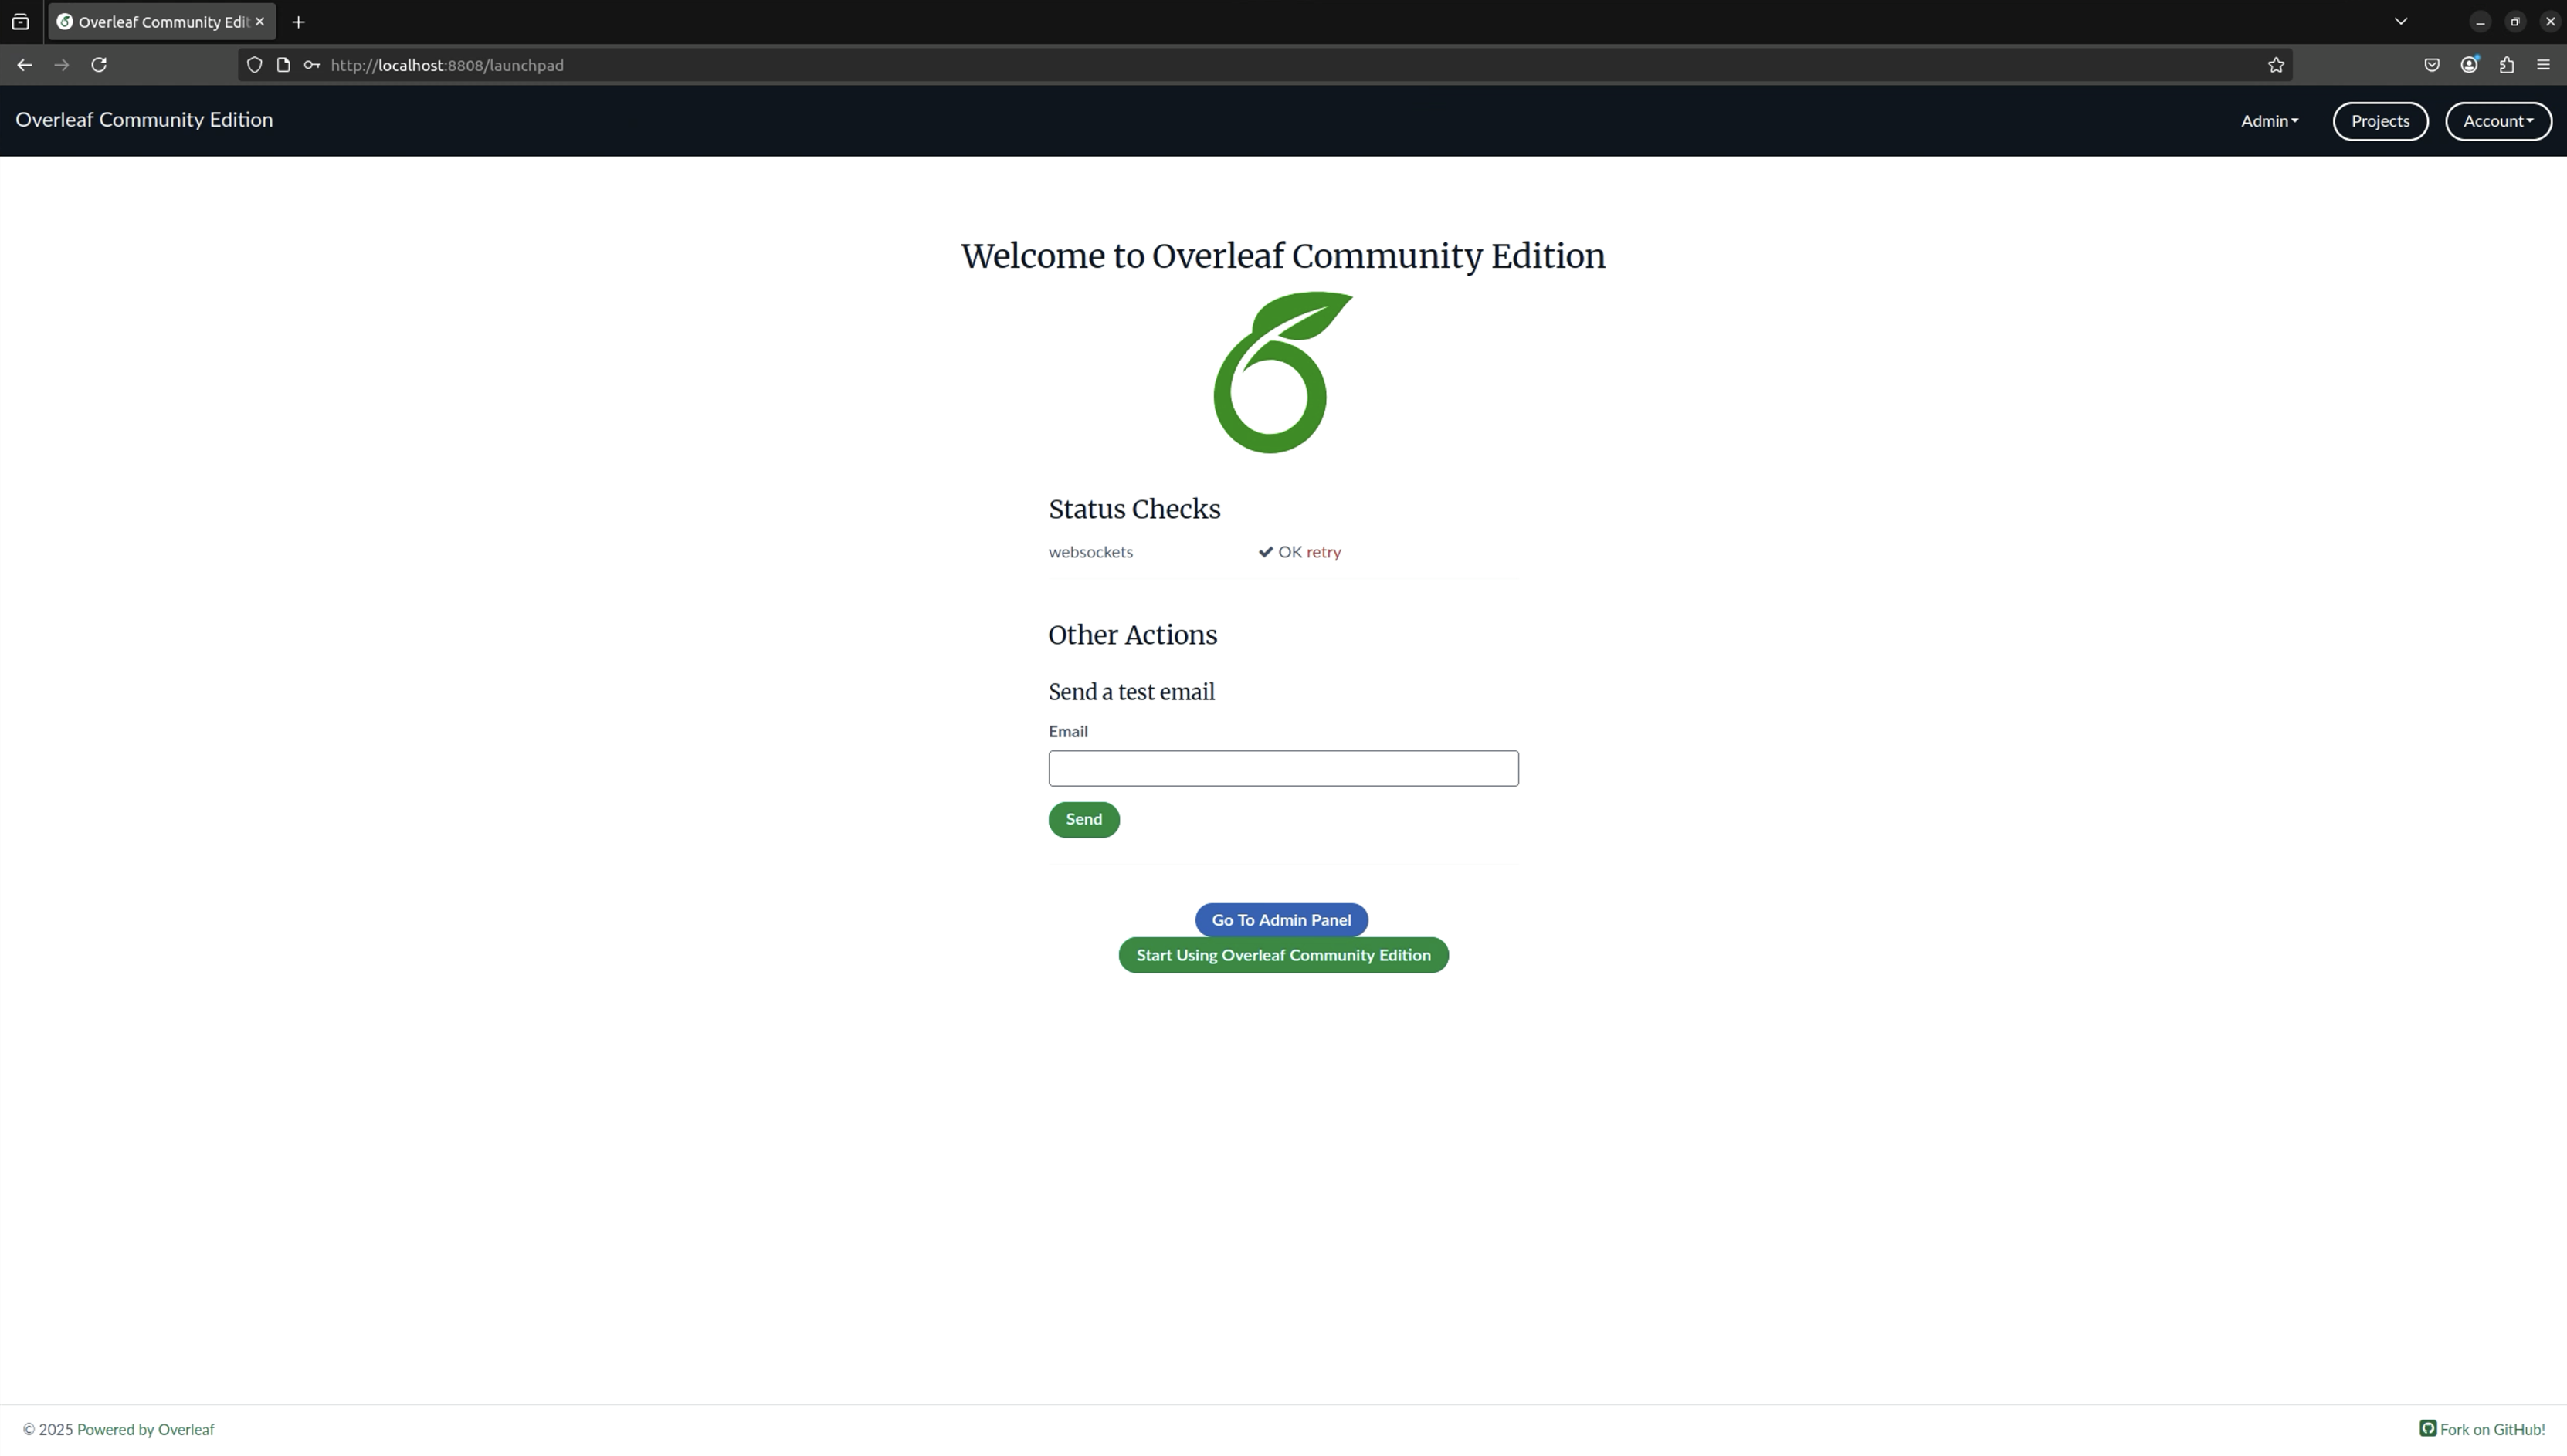
\includegraphics[width=0.8\linewidth]{images/Pasted image 20250307160656.png}
\end{figure}

その後,英語の簡単な文書を作成できる.

\begin{figure}[H]
    \centering
    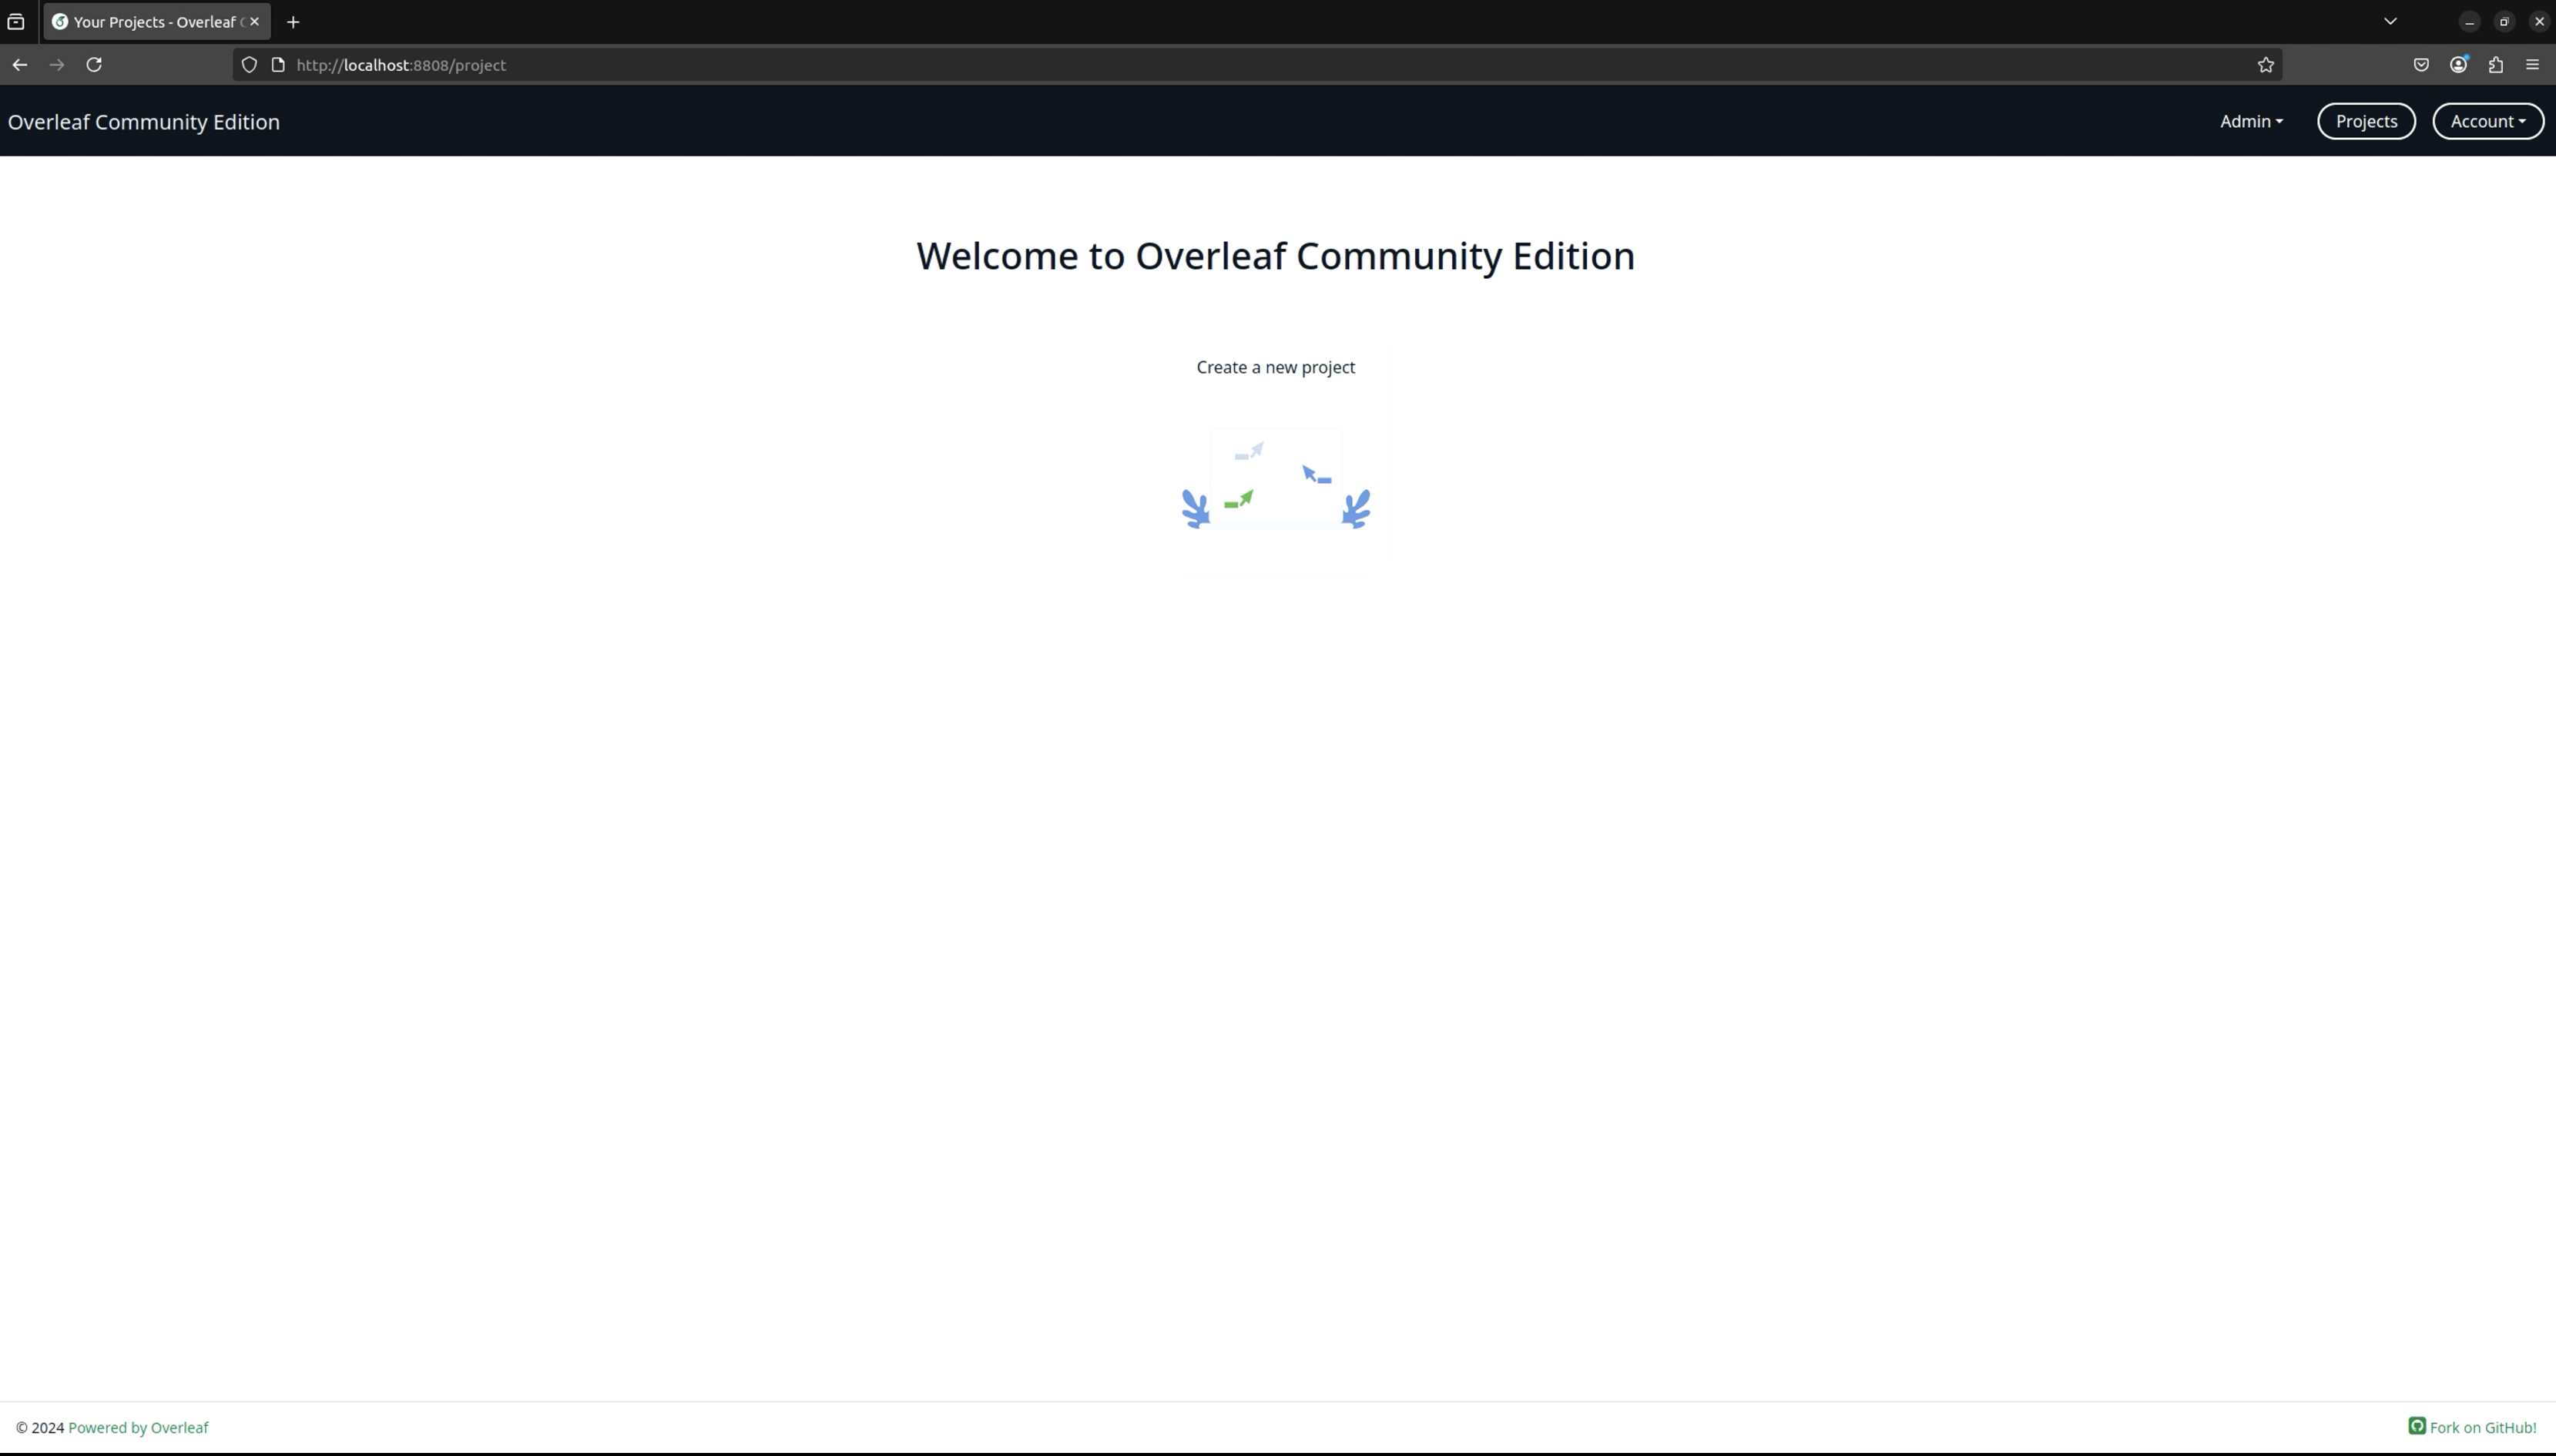
\includegraphics[width=0.8\linewidth]{images/Pasted image 20250307160922.png}
    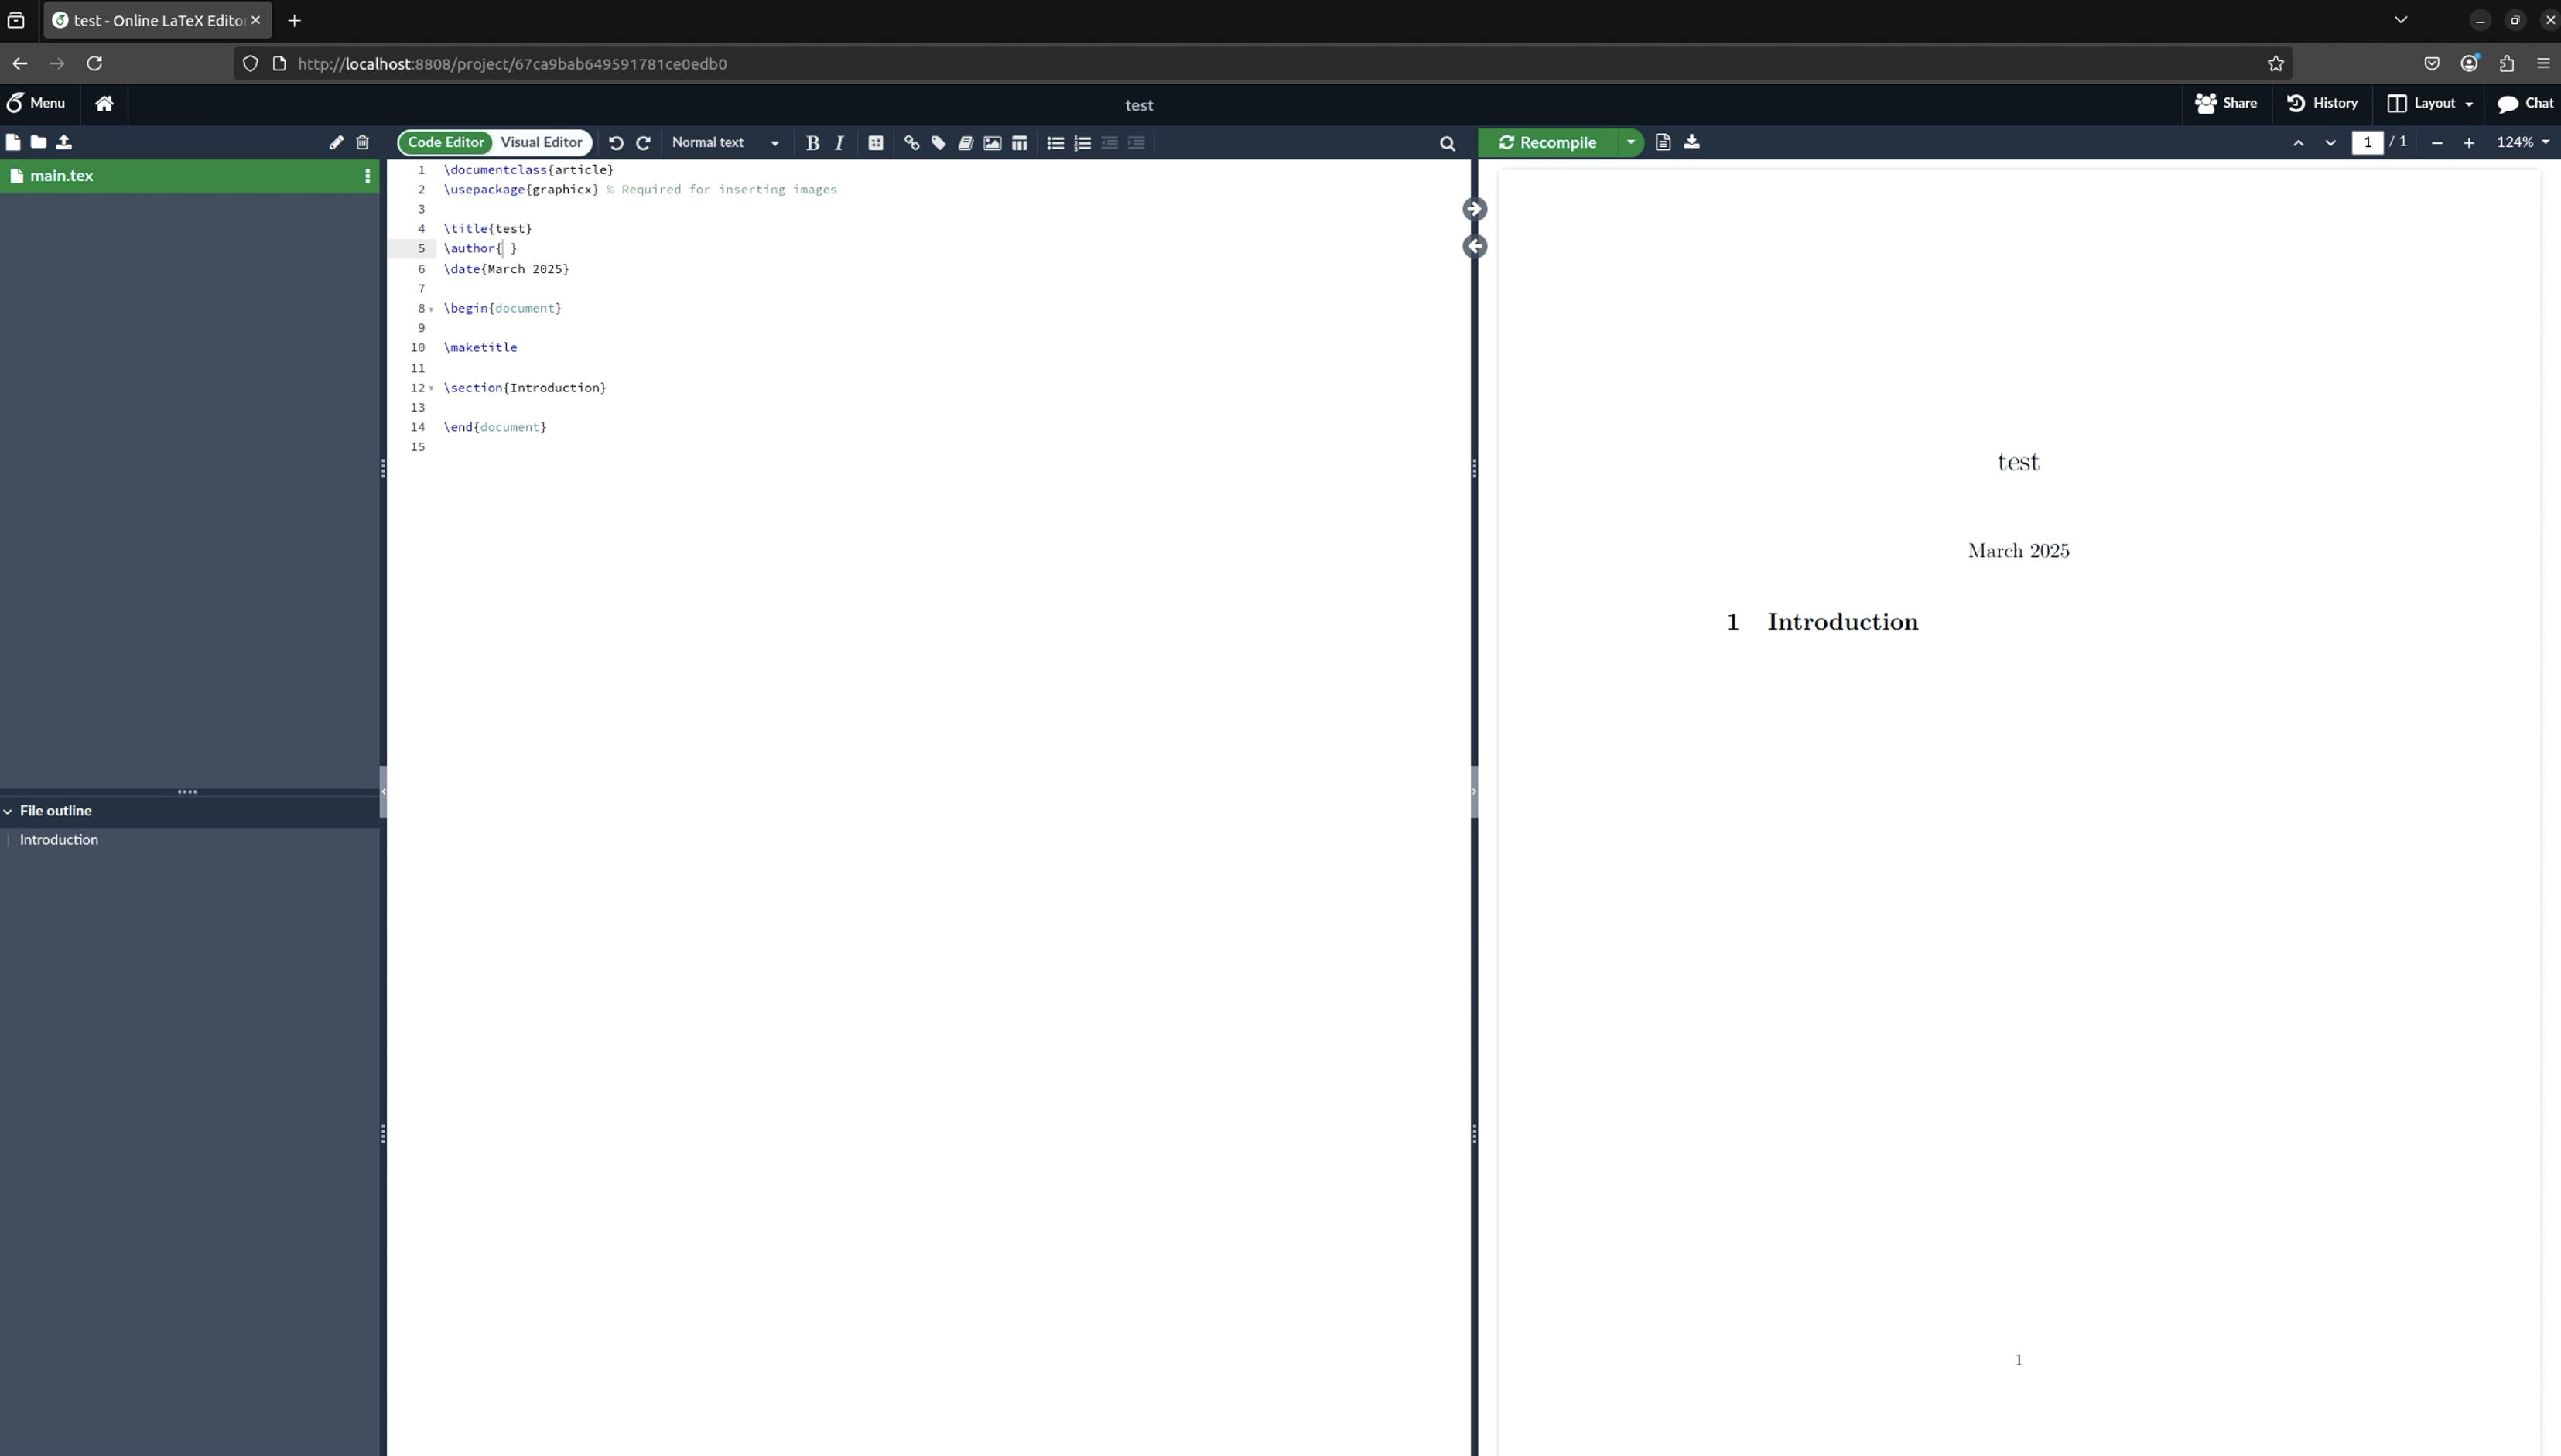
\includegraphics[width=0.8\linewidth]{images/Pasted image 20250307161002.png}
\end{figure}

\subsection{完全なTeXLiveとCJK言語サポートのデプロイ}
デフォルトのShareLaTeXイメージには最小限のTeXLiveのみが含まれている.完全版をインストールするには以下の手順に従うこと:

\begin{enumerate}
\item コンテナ内部でコマンドラインに入る
\begin{lstlisting}[language=bash]
docker exec -it sharelatex-test /bin/bash
\end{lstlisting}

\item \texttt{tlmgr}の更新と完全版TeXLiveのインストール
\begin{lstlisting}[language=bash]
tlmgr update --self
tlmgr install scheme-full
\end{lstlisting}
完全なTeXLiveのインストールには長時間を要する.ネットワーク環境とサーバ性能に応じて,コーヒーを飲むか昼食を取ることを推奨する.

\item CJK文字エンコーディングライブラリと言語サポートのインストール
\begin{lstlisting}[language=bash]
apt update
apt install -y latex-cjk-all texlive-lang-chinese texlive-lang-japanese texlive-lang-korean texlive-lang-english fonts-noto-cjk
\end{lstlisting}
\end{enumerate}

\paragraph{Google Notoフォントについて}
Google Notoフォント(Noto CJK)は中国語・日本語・韓国語の文字を統一デザインでサポートするオープンソースフォントである.以下の名前に対応している:
\begin{itemize}
\item 日本語:Noto Sans CJK JP/Noto Serif CJK JP
\item 簡体字中国語:Noto Sans SC/Noto Serif SC
\item 繁体字中国語:Noto Sans TC/Noto Serif TC
\item 韓国語:Noto Sans KR/Noto Serif KR
\end{itemize}

\paragraph{XeLaTeXの設定}
\LaTeX 文書でCJK文字を正しくレンダリングするには:
\begin{itemize}
\item 左上メニューからコンパイルツールを\texttt{XeLaTeX}に変更する
\item 文書先頭にパッケージを追加する:
\begin{lstlisting}[language=TeX]
\usepackage{xeCJK}
\end{lstlisting}
\end{itemize}

\begin{figure}[H]
    \centering
    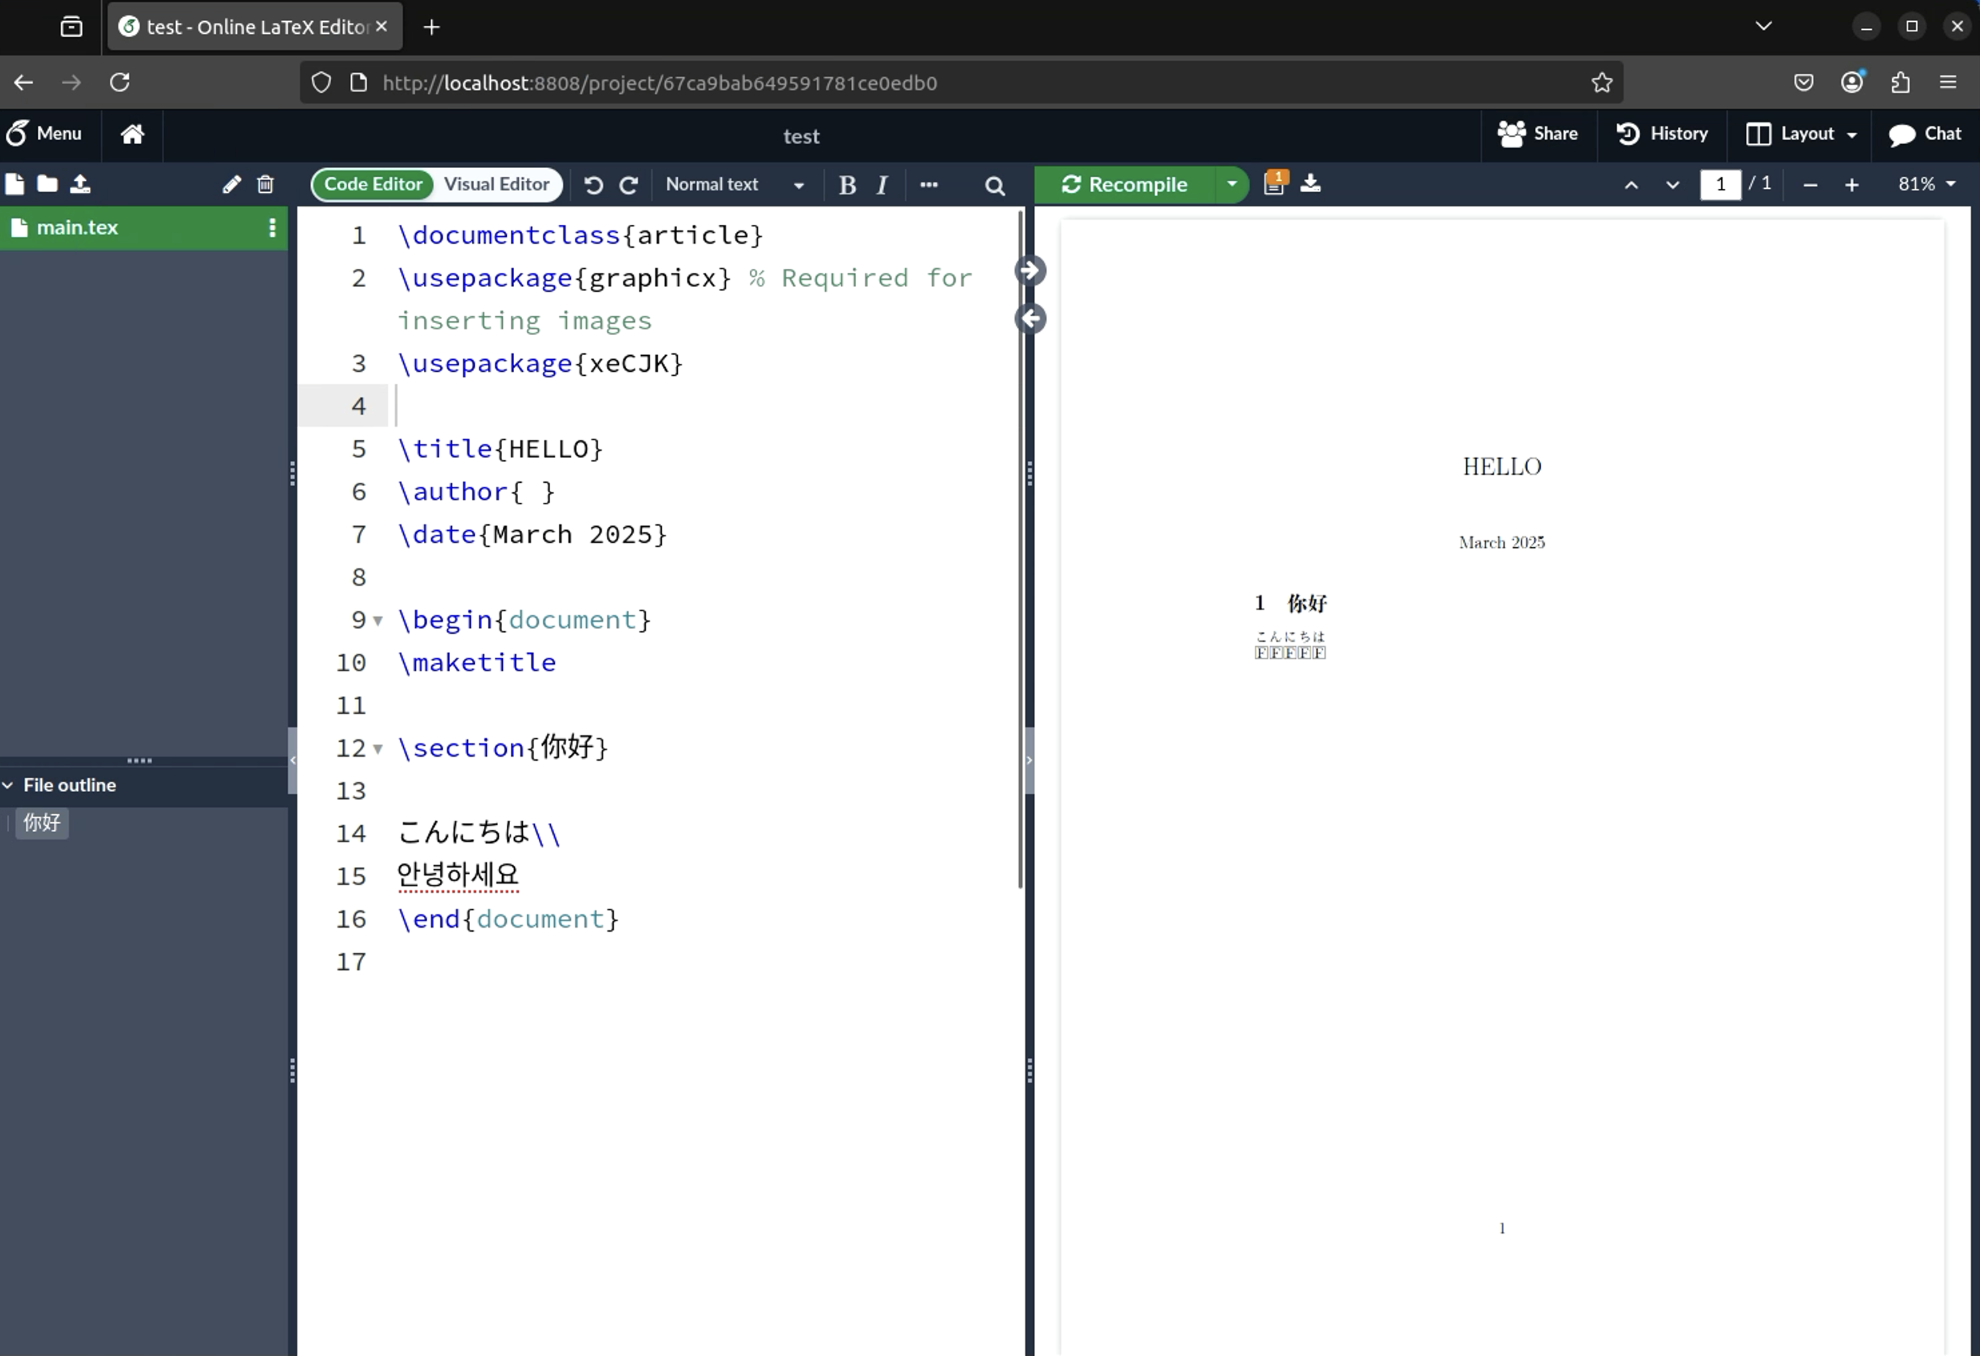
\includegraphics[width=0.8\linewidth]{images/Pasted image 20250307175237.png}
\end{figure}

\paragraph{韓国語の追加設定}
韓国語を使用する場合はフォントを明示的に指定する必要がある:
\begin{lstlisting}[language=TeX]
\usepackage{kotex}
\setmainhangulfont{Noto Serif CJK KR}
\end{lstlisting}

\begin{figure}[H]
    \centering
    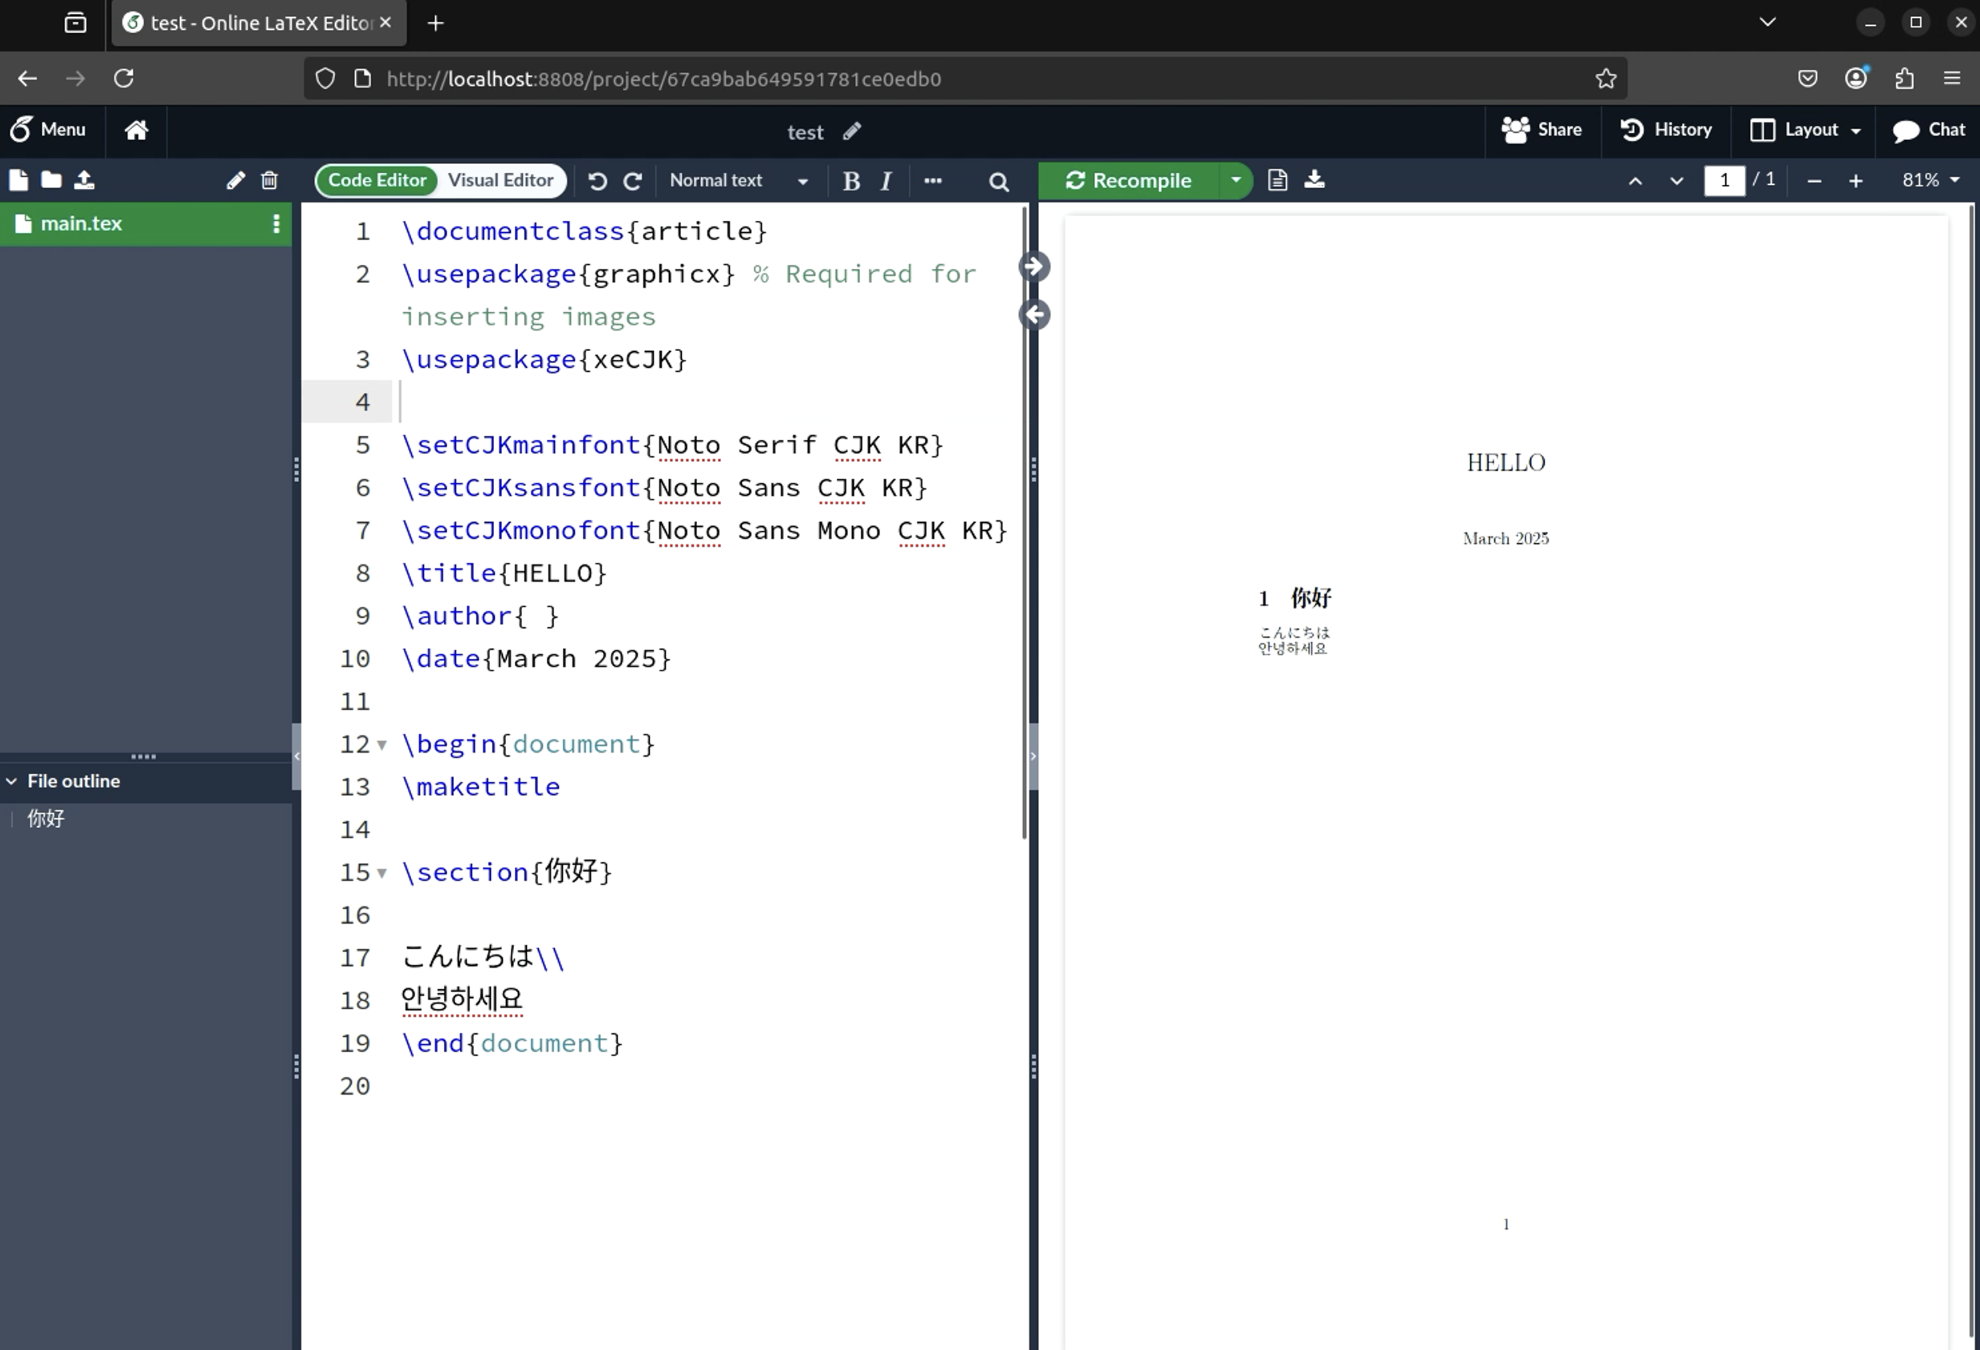
\includegraphics[width=0.8\linewidth]{images/Pasted image 20250307180333.png}
\end{figure}

また,日本語や中国語が正しく表示できない場合は,対応するフォントを指定することで正常に表示できる.
    
\paragraph{その他の機能}
ファイル管理やマルチユーザー協業機能など,その他の実用的な機能はOverleaf公式Web版と同様である.ただし,SandBoxなどの高級機能は含まれていない.


\section{Dockerコンテナを用いた開発環境の構築}
続いて統合開発環境(IDE)のDocker連携機能について説明する.JetBrains社の各種IDEやMicrosoft社のVisual Studioなど,多くのIDEがDocker開発機能を統合または拡張可能だが,これらは通常追加のDockerリモートサポート購入が必要である.研究チームがクラスタやサーバ上でDockerを運用する場合,必ずしも最適な解決策とは言えない.そこで,Microsoft社が提供するVisual Studio Code(以下VS Code)を推奨する.

\subsection*{Visual Studio Codeについて}
VS Codeはオープンソースの軽量エディターで,以下の特徴を持っている:
\begin{itemize}
\item クロスプラットフォーム(Windows/macOS/Linux)対応
\item 豊富な拡張機能エコシステム
\item 組み込みターミナルとGit統合
\item 無料で商用利用可能
\end{itemize}

VS Codeのインストール手順は容易なため,ここでは割愛する.次に,公式ガイド「\href{https://code.visualstudio.com/docs/containers/overview}{Docker in Visual Studio Code}」を参照し,VS CodeにDocker拡張機能をインストールすること.

\subsection{PyTorchコンテナの実行例}
\begin{lstlisting}[language=bash]
docker run --name pytorch-test --mount type=bind,src=/home/username,dst=/root/ --gpus all --ipc=host -it nvcr.io/nvidia/pytorch:xx.xx-py3
\end{lstlisting}

\paragraph{コマンドパラメータ解説}
\begin{itemize}
\item \texttt{--mount type=bind,src=/home/username,dst=/root/} :
ディレクトリマウント.ホストOSの\texttt{/home/username}ディレクトリをコンテナ内の\texttt{/root/}にバインドマウント(双方向同期)する.

\item \texttt{--ipc=host} :
IPC名前空間共有.コンテナがホストOSのプロセス間通信(Inter-Process Communication)リソースにアクセス可能にする(共有メモリを使用するアプリケーションに必須).

\item \texttt{--gpus all} :
GPUデバイス割当.NVIDIA GPUをコンテナに全デバイス公開する(NVIDIA Container Toolkitの事前インストールが必要).

\item \texttt{nvcr.io/nvidia/pytorch:xx.xx-py3} :
コンテナイメージ指定.\href{https://docs.nvidia.com/deeplearning/frameworks/support-matrix/index.html}{NVIDIA NGCカタログ}で提供されるPyTorch公式イメージ(\texttt{xx.xx}はCUDA/PyTorchバージョンの組み合わせ).
\end{itemize}


\paragraph{\texttt{--mount}と\texttt{--volume}の違い}
前章で使用した\texttt{-v}(\texttt{--volume}の省略形)との主な差異:
\begin{itemize}
\item \texttt{--volume}: Docker管理のボリュームを使用(データ暗号化可能・外部アクセス困難)→ アプリ配布/機密データ向け
\item \texttt{--mount}: ホストOSのファイルシステムを直接マウント(双方向リアルタイム同期)→ 開発環境向け
\end{itemize}

\subsection{VS Codeとの連携手順}
コンテナ起動後,VS CodeのDocker拡張機能から該当コンテナを右クリックし「Attach Visual Studio Code」を選択する.新規ウィンドウが開いたら,作成済みのコンテナを選択する.

\begin{enumerate}
\item プロジェクトディレクトリ(Sec.5.1で取得したディレクトリ)を開き,\texttt{./notebook/mnist.ipynb}ファイルを選択する
\item カーネル選択で「Python Environments」→「Global Env」を指定する
\item 自動表示されるポップアップから「Python + Jupyter拡張機能」をインストールする
\item インストール完了後,再びファイルを開いてカーネルを選択する
\end{enumerate}

\paragraph{\texttt{torch}インポートエラー/GPU認識不良時}
コンテナ内で\texttt{nvidia-smi}を実行した際,以下のエラーが発生する場合:
\begin{lstlisting}
% nvidia-smi
Failed to initialize NVML: Unknown Error
\end{lstlisting}
解決策:
\begin{itemize}
\item コンテナを再起動する(前章のGPUデバイスマウント手順を再確認する)
\item NVIDIAドライバのバージョンとコンテナの互換性を確認する
\end{itemize}

これでJupyter Notebookの編集と実行ができる.以降の操作はVS Code上で実施すること.